%************************************************
\chapter{Antiferromagnetic resonance in a Rashba honeycomb antiferromagnet} % $\mathbb{ZNR}$\
%************************************************
In this Chapter we investigate the role of Rashba spin orbit interaction on the exchange Gilbert damping in a honeycomb antiferromagnet. We find that when the band splitting due to spin orbit is much smaller than the disorder-induced level broadening, disorder averaging will lead to a titanically large value of exchange Gilbert damping, which reflects the fact that it requires many scattering events to randomize the spin of a conducting electron. In the opposite limit where the spin-split bands can indeed be resolved the damping becomes suppressed by many orders of magnitude. Furthermore the damping becomes ultimately anisotropic which was the topic of the previous Chapter. We report that in the antiferromagnetic resonance spectrum we can directly see the effect of the exchange damping. In the large damping regime the magnetic system becomes overdamped and no resonance can be observed. The resonance appears to get a maximum value when the spin-orbit coupling has a value equal to the inverse momentum life-time of conducting electrons. 

\vfill
Parts of this Chapter are under preparation for submission to Physical Review Letters\clearpage



% In this Chapter we investigate the role of Rashba spin orbit interaction on the exchange Gilbert damping in a honeycomb antiferromagnet. We find that when the band splitting due to spin orbit is much smaller than the disorder-induced level broadening, disorder averaging will lead to a titanically large value of exchange Gilbert damping, which reflects the fact that it requires many scattering events to randomize the spin of a conducting electron. In the opposite limit where the spin-split bands can indeed be resolved the damping becomes suppressed by many orders of magnitude. Furthermore the damping becomes ultimately anisotropic which was the topic of the previous Chapter. We report that in the antiferromagnetic resonance spectrum we can directly see the effect of the exchange damping. In the large damping regime the magnetic system becomes overdamped and no resonance can be observed. The resonance appears to get a maximum value when the spin-orbit coupling has a value equal to the inverse momentum life-time of conducting electrons. 

% Before introducing our model system, let us briefly make a few general observations about conducting antiferromagnets. Consider two magnetization vectors $\bb{m}_\text{A}$ and $\bb{m}_\text{B}$ on two sublattices of a antiferromagnet and furthermore conducting electrons with spin-polarizations $\bb{s}_\text{A(B)}$. An exchange interaction $\Delta$ couples the spin degree of freedom with the magnetization on each sublattice locally, leading to the following equations of motion on magnetization vectors
% \beml
% \label{basicEQ}
% \begin{align}
% \dot{\bb{n}}^\textrm{A}  & = \bb{H}^\textrm{A}\times\bb{n}^\textrm{A}  + (J\mathcal{A}/\hbar)\,\bb{n}^\textrm{A}\times \bb{s}^\textrm{A},\\
% \dot{\bb{n}}^\textrm{B} & = \bb{H}^\textrm{B}\times\bb{n}^\textrm{B} +(J\mathcal{A}/\hbar)\,\bb{n}^\textrm{B}\times \bb{s}^\textrm{B},
% \end{align}
% \eml
% where $\bb{H}$ is an effective field, $\mathcal{A}$ is the area of the unit cell, and $J$ and $\hbar$ are the (local) exchange energy and reduced Planck's constant ($h/2\pi$) respectively. 

% We are interested in the response tensor $\alpha$ relating the spin-polarizations with the time-derivative of magnetizations
% \begin{equation}
% \label{eq:basicGilbert}
%     \begin{pmatrix}
%     \bb{s}_\text{A} \\ \bb{s}_\text{B}
%     \end{pmatrix}
%     =
%     \begin{pmatrix}
%     \alpha_{11}  &  \alpha_{12} \\ \alpha_{21}  &  \alpha_{22}
%     \end{pmatrix}
%     \begin{pmatrix}
%     \partial_t \bb{m}_\text{A} \\ \partial_t\bb{m}_\text{B}
%     \end{pmatrix}.
% \end{equation}
% The first observation we make is that the presence of sub-lattice-symmetry (the interchanging of the labels $A\leftrightarrow B$) necessarily leads to $\alpha_{11}=\alpha_{22}=\alpha_0$ and $\alpha_{11}=\alpha_{22}=\alpha'$. As written in the introduction when spin-orbit interaction is absent the angle between magnetizations $\bb{m}_\text{A}$ and $\bb{m}_\text{B}$ must be conserved. By inserting Eq.~(\ref{eq:basicGilbert}) into Eq.~(\ref{basicEQ}) we immediately find that $\alpha_0=\alpha'$ so that the damping tensor can be entirely described by the single number $\alpha_0$. Next we introduce the non-staggered and staggered magnetizations 
% \begin{equation}
%     \bb{m} = \bb{m}_\text{A} + \bb{m}_\text{B}, \quad \bb{n} = \bb{n}_\text{A} - \bb{n}_\text{B},
% \end{equation}
% and their equations of motion
% \begin{align}
%     \partial_t{\bb{n}}   & = \bb{H}\times\bb{n}  + \alpha_0 J\mathcal{A}/\hbar\,\bb{n}\times \partial_t\bb{m}\\
%     \partial_t{\bb{m}}   & = \bb{H}\times\bb{m}  + \alpha_0 J\mathcal{A}/\hbar\,\bb{m}\times \partial_t\bb{m},
% \end{align}
% from which one can immediately see that the modulus of both $\bb{m}$ and $\bb{n}$ are conserved. Alternatively one can reach the same conclusion by noting that $\partial_t (\bb{m}_\text{A}\cdot\bb{m}_\text{B}) = \partial_t (m^2-n^2) = 0$ and that by construction $n^2+m^2=1$, from which it immediately follows that $\bb{m}\cdot\partial_t\bb{m} = \bb{n}\cdot\partial_t\bb{n} = 0$. 


\section{Role of vertex-corrections on the asymptotic behavior of $\alpha_{m,zz}$ and $\alpha_{m,\parallel}$}
It was shown in the previous Chapter that when $\lambda=0$ the damping tensor is isotropic, while in the limit $\lambda\tau\gg 1$ we find an ultimate anisotropy where $\alpha_{m,zz}$ vanishes completely. In the this limit, the spin-split bands are completely resolved and certain spin-flip processes corresponding to interband transitions become forbidden. A more quantitative discussion on the role of disorder averaging will be presented in this section.

It will turn out that the role of vertex-corrections on the components of the $\alpha_m$ tensor has a profound effect when $\lambda\tau/\hbar\ll1$, but negligible when $\lambda\tau/\hbar\gg1$. 

In the limit $\Delta_\text{sd}$ we are able to obtain concise and exact analytical formulas, that we present first. As shown in Eqs.~(\ref{chap03:gilbert}), (exchange) Gilbert damping can be fully described by two parameters $\alpha_m^{\parallel}$ and $\gamma$: 
\begin{equation}
\bb{s}^+ = \alpha_m^{\parallel}\, \dot{\bb{m}}_{\parallel} + \gamma\, \Gamma_{mm},
\end{equation}where $\Gamma_{mm}$ was a rather complicated vector form involving both $\dot{\bb{m}}_{\parallel}$ and $\dot{\bb{m}}_\perp$. For the present discussion we find it more convenient to remove the term proportional to $\dot{\bb{m}}_{\perp}$ from $\Gamma_{mm}$ completely, i.e.
\begin{equation}
\bb{s}^+  = \alpha_m^{\parallel}\,\dot{\bb{m}}_\parallel + \alpha_m^{\perp}\,\dot{\bb{m}}_{\perp} + \gamma'\Gamma'_{mm} 
\end{equation}and focus on $\alpha_m^{\parallel}$ and $\alpha_m^{\perp}$. 

As mentioned throughout this Thesis, disorder averaging involves (i) replacing clean Green's functions with disorder-averaged Green's functions in the Born approximation and (ii) summing different diagrams in the (diffusive) ladder approximation (i.e. Figure~\ref{sd:fig:diagrams}b). Let us annotate the parallel-to-the-plane and perpendicular-to-the-plane Gilbert damping coefficients with a superscript $(i)$ that denotes that we summed over all diagrams with $\leq i$ disorder lines inserted. Physically, it means averaging over various disorder ensembles where the electron scatters $i$ number of times. 

Let us first consider first the ``bare bubble'' contribution which describes an electron entering and exiting the system without a single scattering event
\begin{align}
    \alpha_{m}^{\perp\,(0)} =  & \frac{\varepsilon\tau}{\hbar} \frac{1-(\lambda/2\varepsilon)^2}{1+(\lambda\tau)^2},\\
    \alpha_{m}^{\parallel\,(0)} =  & \frac{\varepsilon\tau}{\hbar}\left(\frac{1}{2}\frac{3+2(\lambda\tau/\hbar)^2}{1+(\lambda\tau/\hbar)^2}-\frac{2}{(4-\lambda/\varepsilon)^2}\right),
\end{align}
where one can immediately see the asymptotic behavior for large and small values of $\lambda\tau$:
\begin{align}
    \alpha_{m}^{\perp\,(0)}  & = \frac{\epsilon\tau}{\hbar}\begin{cases}
    1  +\mathcal{O}(\lambda/\varepsilon)  & \text{ for }\lambda\tau/\hbar\ll1\\
    \hbar/(\lambda\tau)^2 & \text{ for }\lambda\tau/\hbar\gg1
    \end{cases},\\
    \alpha_{m}^{\parallel\,(0)}  & = \frac{\epsilon\tau}{\hbar}\begin{cases}
    1  +\mathcal{O}(\lambda/\varepsilon)  & \text{ for }\lambda\tau/\hbar\ll1\\
    1/2 + \hbar/2(\lambda\tau)^2 & \text{ for }\lambda\tau/\hbar\gg1.
    \end{cases}
\end{align}
Evidently, the exchange damping transitions from fully isotropic to ultimately anisotropic when changing the limits $\lambda\tau\ll1$ to $\lambda\tau\gg1$. 
Including a small number of scattering events in the calculation we find an interesting modification:
\begin{align}
	\label{eq:perpi}
    \alpha_{m}^{\perp\,(i)}  & = \frac{\epsilon\tau}{\hbar}\begin{cases}
    i + \mathcal{O}(\lambda/\varepsilon)  & \text{ for }\lambda\tau/\hbar\ll1\\
    \hbar/(\lambda\tau)^2 & \text{ for }\lambda\tau/\hbar\gg1,
    \end{cases}\\
    \label{eq:parai}
    \alpha_{m}^{\parallel\,(i)}  &  = \frac{\epsilon\tau}{\hbar}\begin{cases}
    i + \mathcal{O}(\lambda/\varepsilon)  & \text{ for }\lambda\tau/\hbar\ll1\\
    1-(1/2)^{i+1}+\mathcal{O}(\hbar/(\lambda\tau)^2) & \text{ for }\lambda\tau/\hbar\gg1.
    \end{cases}
\end{align}
In the large $\lambda\tau$ limit perpendicular-to-the-plane component of the Gilbert damping is unchanged by scattering events, whereas the parallel component quickly converges to the value of $\varepsilon\tau$. In the opposite limit, where the components remain isotropic with respect to each other, the components have a profound sensitivity to scattering events. Each scattering event contributes a value of $1\times\varepsilon\tau$ to the damping coefficient. While at a first glance it appears as strong sensitivity to impurities, it in reality reflects a long spin-life time: many scattering events are required to randomize the spin of an electron. 

In a truly diffusive system one should take the limit $i\rightarrow\infty$, in which case the tensor components are given by
\begin{align}
\label{eq:alphaperpzerodelta}
    \alpha_{m}^{\perp}\equiv\alpha_{m}^{\perp\,(\infty)}  & = \frac{\epsilon \tau}{\hbar}\, 2\frac{1+\lambda^2\tau^2}{\lambda^2\tau^2},\\
  \label{eq:alphaparallelzerodelta}  \alpha_{m}^{\parallel}\equiv\alpha_{m}^{\parallel\,(\infty)}  & = \frac{\varepsilon\tau}{\hbar}\,\frac{1}{\lambda^2\tau^2}.
\end{align}

We plot the functions of $\alpha_{m,zz(\parallel)}^{(i)}$ for $i=0,1,2$ and $i\rightarrow\infty$ in Fig.~\ref{fig:alpha_plot}. 
\begin{figure}
    \centering
    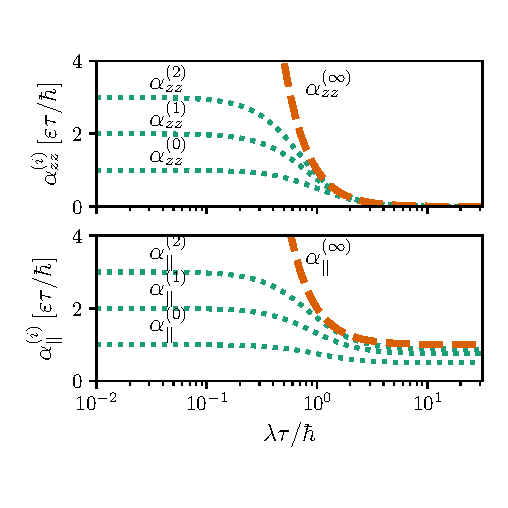
\includegraphics[width=\linewidth]{gfx/Chapter04/alpha_plot2}
    \caption{The first three scattering contributions $\alpha_{m,zz}^{(i)}$, $i=0,1,2$ (green, dotted) and the fully vertex corrected $\alpha_{m,zz}^{(\infty)}$ (orange, dashed) as a function of $\lambda \tau$. }
    \label{fig:alpha_plot}
\end{figure}

We find that indeed in the limit $\lambda\tau\gg1$ the exchange Gilbert damping becomes ultimately anisotropic where $\alpha_{m}^{\perp}$ becomes vanishingly small. Moreover, we find a substantial drop of $\alpha_{m,\parallel}$ for increasing values of $\lambda\tau$, that can reach a difference of many orders of magnitude. 

We note that a large value for damping corresponds to an overdamped regime, which we will explain in details in the next section. The direct exchange parameter $\Delta$ leads to a cut-off of the $1/(\lambda\tau)$ singularity in the limit $\lambda\tau\ll1$:

\begin{align}
\label{eq:alphapara}
    \alpha_{\parallel} &= 
    \frac{\varepsilon\tau\Delta}{2}\,  \begin{cases}
        \frac{4}{3}\frac{\varepsilon^2+\Delta^2}{\Delta^2}
            &\quad \text{for } \lambda\tau        \ll \Delta/\varepsilon\\
        2\frac{1+(\lambda\tau)^2}{(\lambda\tau)^2}
            &\quad \text{for } \lambda\tau \gg \Delta/\varepsilon 
    \end{cases}\\
    %
    \label{eq:alphaperp}
    \alpha_{\perp} &= \frac{\varepsilon\tau\Delta}{2}\,
    \begin{cases}
        \frac{2}{3}\frac{\varepsilon^2+\Delta^2}{\Delta^2}
            \quad\quad &\text{for } \lambda\tau        \ll \Delta/\varepsilon\\
        \frac{1}{(\lambda\tau)^2}
            \quad &\text{for } \lambda\tau \gg \Delta/\varepsilon 
    \end{cases}
\end{align}
%%%
%%%
\begin{figure}
    \centering
    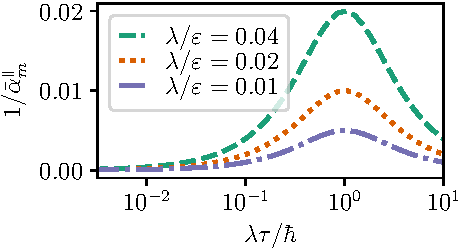
\includegraphics[width=0.75\linewidth]{gfx/alpha_full}
    \caption{Fully vertex-corrected parallel and perpendicular Gilbert damping. In the limit $\lambda\tau\ll1$ we find the limiting behavior $(4)2(\Delta^2+\varepsilon^2)/2$ for $\alpha_{\perp(\parallel)}$. When $\lambda\tau\ll 1$ and $\lambda\tau\gg\Delta/\varepsilon$ we find a scaling behavior $\alpha_{\perp(\parallel)}=(1)2/\lambda^2\tau^2$. Note the use of log-scale on both vertical and horizontal axis. The plot is obtained using $\varepsilon\tau=50$ and $\Delta\tau=0.1$. }
    \label{fig:alpha_plot}
\end{figure}



Note that in Eqs.~(\ref{eq:alphapara,eq:alphaperp}) in the limits $\lambda\tau\ll 1$ and $\lambda\tau\gg1$ we find different magnitudes for the anisotropy:
\begin{equation}
	\frac{\alpha_{\parallel}}{\alpha_{\perp}} = \begin{cases}
    	2 
        	& \quad \text{for } \lambda\tau\ll 1\\
        (\lambda\tau)^2
        	& \quad \text{for } \lambda\tau\gg 1.
    \end{cases}
\end{equation}
The second limit is what we referred to as the giant Gilbert damping anisotropy in the previous Chapter. The factor of two in the former limit is well known in the literature (e.g. \cite{DYAKONOV1986, aronov_spin_1983, averkiev_spin_2002, burkov_theory_2004}). Note that this factor is absent in Eqs.~(\ref{eq:perpi},\ref{eq:parai}) and only appears in the diffusive limit. 

It is worth reminding the reader that we use a particular model to describe spin-relaxation. The relaxation is fully described by the combination of spin-orbit interaction and scattering of electrons of an impurity potential. A Rashba-type spin-orbit interaction is described as electrons moving through an asymmetric crystal potential. In the electron frame they experience a momentum-dependent magnetic field that leads to the spin-splitting of the conduction band, which is the case studied by Dyakonov and Perel \cite{dyakonov1972spin, DYAKONOV1986} and the spin-relaxation mechanism they introduced is named after them. 

In the presence of a spin-orbit field, the spin of the electron will precess around the direction of that field with a certain frequency $\Omega_s$. We can then distinguish two cases: (i) $\Omega_s \tau < 1$ where between each scattering event the spin does not have enough time to deviate from its initial spin direction in a significant manner, and (ii) $\Omega_s\tau>1$ where the electron spin can precess freely between each collision. 
Dyakonov-Perel then gives the following spin-relaxation rates $1/\tau_s$
\begin{equation}
	1/\tau_s \sim \begin{cases}
    	\langle \Omega^2_s\tau\rangle & \quad\text{for  } \Omega_s\tau < 1\\
        1/\tau  &\quad \text{for  }  \Omega_s\tau>1,
    \end{cases}
\end{equation}
where $\langle\cdots\rangle$ denotes momentum averaging. Both cases can be understood as follows. In a time-scale set by $\Omega_s$ we find that in the first case the electron experiences many scattering events. Due to the random motion involved, the electrons experience as if moving through a randomly changing magnetic field and as such lose their spin-orientation in a diffusive manner. Each scattering event contributes to the squared precession deviation with $(\Omega_s\tau)^2$, and the spin-life time may be defined as the time needed for the squared precession deviation to be of the order of unity, i.e. $1\tau_s\sim \Omega_s^2\tau$. Because the electrons are confined in two-dimensions the random spin-orbit field is always directed in-plane, leading to a decrease in the in-plane spin-relaxation rate by a factor of two compared to the out-of-plane spin-relaxation rate \cite{DYAKONOV1986, aronov_spin_1983, averkiev_spin_2002, burkov_theory_2004}. 

In the second case on the other hand, the spin can freely rotate around the magnetic field between each collision and this orientation is only lost on the same time scale as momentum is lost, i.e. on the time scale of $\tau$ \cite{aronov_spin_1983, dyakonov_spintronics_2004}, leading to $1/\tau_s \sim 1/\tau$.

The mechanism leading to Dyakonov-Perel relaxation of the electron's spin can be generally understood quite classically \cite{dyakonov_spintronics_2004}. In the regime $\Omega_s \tau > 1$ we found however that $\alpha_m^{\perp}$ does not follow Dyakonov-Perel and is a result of forbidden interband transitions. 

It is also important to note that the relaxation rate $1/\tau_s\sim 1/\tau$ that we find for $\alpha_m^{\parallel}$ in the regime $\Omega_s \tau > 1$ also appears in processes described by the Elliot-Yafet mechanism \cite{elliott_theory_1954, yafet_g_1963}, where spin-orbit coupling leads to the change of spin due to scattering events. This contribution was calculated in Ref. \cite{huertas-hernando_spin-orbit-mediated_2009} for intrinsic graphene with Rashba spin-orbit (but without the local exchange $\Delta$) showing $1/\tau_s \sim \lambda^2/\varepsilon^2 \times 1/\tau $ and has therefore a negligible contribution in the high-energy regime (i.e. $\varepsilon \gg \lambda + \Delta$) that we consider.
%%%
%%%

We plot the functions of $\alpha_{m,zz(\parallel)}^{(i)}$ for $i=0,1,2$ and $i\rightarrow\infty$ in Fig.~\ref{fig:alpha_plot}. 
\begin{figure}
    \centering
    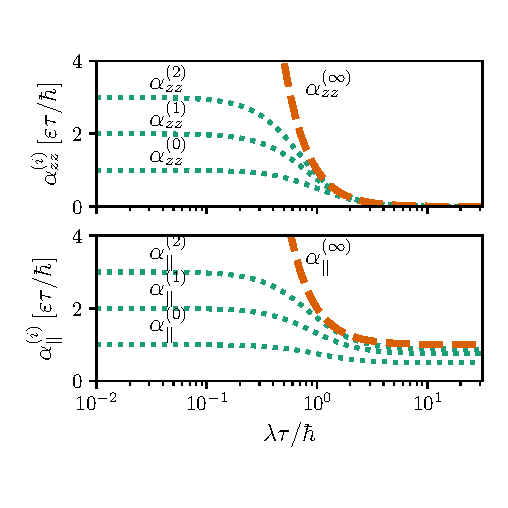
\includegraphics[width=\linewidth]{gfx/Chapter04/alpha_plot2}
    \caption{The first three scattering contributions $\alpha_{m,zz}^{(i)}$, $i=0,1,2$ (green, dotted) and the fully vertex corrected $\alpha_{m,zz}^{(\infty)}$ (orange, dashed) as a function of $\lambda \tau$. }
    \label{fig:alpha_plot}
\end{figure}
% We find that indeed in the limit $\lambda\tau\gg1$ becomes ultimately anisotropic where $\alpha_{m,zz}$ becomes vanishingly small. Moreover, we find a substantial drop of $\alpha_{m,\parallel}$ for increasing values of $\lambda\tau$, that can reach a difference of many orders of magnitude. 

% We note that a large value for damping corresponds to an overdamped regime, which we will explain in details in the next section. 

% The direct exchange parameter $\Delta$ can be included perturbatively in both overdamped and underdamped regimes. In the overdamped regime,  $\Delta$ merely introduces a cutoff whereas in the underdamped regime a small modification.
% \begin{align}
% \label{eq:alphaparallelzerodelta}
%     \alpha_{m,zz}^{(\infty)}  & = \frac{\epsilon \tau}{\hbar}\, \frac{2}{(2-n_z^2)\lambda^2\tau^2+2\Delta^2/\varepsilon^2},\\
%     \alpha_{m,\parallel}^{(\infty)}  & = \frac{\varepsilon\tau}{\hbar}\,\frac{2(1+\lambda^2\tau^2)}{(2-n_z^2)\lambda^2\tau^2+2\Delta^2/\varepsilon^2}.
% \end{align}
% {\color{blue} Need to find correct coefficients for the underdamped regime ($\lambda\tau\gg1$)}
% that we illustrate in Fig.~\ref{fig:alpha3}.
\begin{figure}
    \centering
    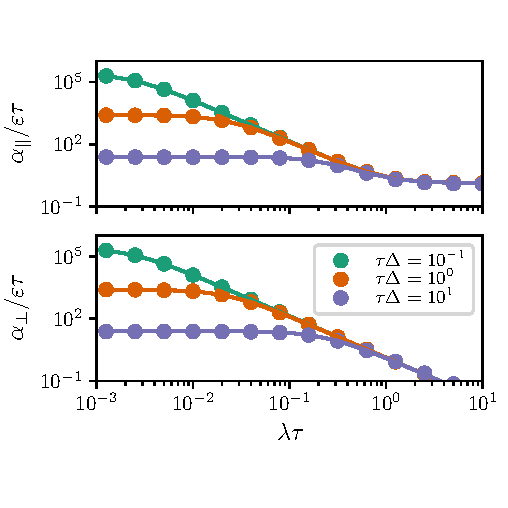
\includegraphics{gfx/Chapter04/alpha_plot1.pdf}
    \caption{Fully dressed damping components $\alpha_{\parallel,\perp}$ as a function of $\lambda\tau$ for three values of $\Delta\tau$. Note the use of log-scale on both horizontal and vertical axes.}
    \label{fig:alpha3}
\end{figure}

The reader might have noticed that in the limit $\lambda\tau\rightarrow0$ Eqs.~(\ref{eq:alphapara,eq:alphaperp}) remain anisotropic, in contradiction to the symmetry analysis presented in the previous Chapter. Indeed, a direct calculation with $\lambda\tau=0$ gives the isotropic damping $\alpha_m^{\perp}=\alpha_m^{\parallel}=(\varepsilon^2+\Delta^2)/\Delta^2$, suggesting a certain scale over which the anisotropy emerges. The numerical analysis illustrated in Figure~\ref{fig:num_test} however reveals that the scale does not depend on the values of $\Delta$ or $\varepsilon$, but rather on the numerical precision instead. This strongly suggests that the transition between isotropic to anisotropic damping occurs at exactly $\lambda=0$. 

However, we defined Gilbert damping as the spin-response to the time-derivative of a \emph{uniform} magnetization. In other words the response was computed in the long wavelength limit $q\rightarrow0$, which is exactly the scale we were looking for. We find therefore that taking the limit $q\rightarrow0$ first and then the limit $\lambda\rightarrow0$ leads to anisotropic Gilbert damping, whereas in the opposite order of limits we find isotropic Gilbert damping.  

\begin{figure}
    \centering
    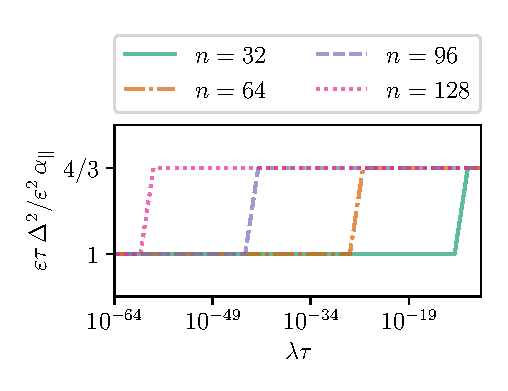
\includegraphics[width=0.75\linewidth]{gfx/numerical_test}
    \caption{The numerical evaluation only yields isotropic Gilbert damping ($\alpha_{\parallel}/\alpha_{\perp}=1$) when $\lambda\tau$ is set below numerical precision. The presented plot is independent of chosen values for $\varepsilon\tau$ and $\Delta\tau$ and only depends on the numerical precision $n$, where $n=32,64,96,128$ is the number of digits contained in each variable during computation (for comparison: a 64 bit, double-precision float generally has about 16 digit precision). }
    \label{fig:num_test}
\end{figure}

%
% uniform modes
%
\section{Uniform modes in collinear ground state}
When subjecting an AFM to an oscillating magnetic field, the localized spins will exhibit a precession parallel to the magnetic field direction. By tuning the magnetic field's frequency to an internal harmonic frequency we can observe resonance. As shown first by Kittel and Keffer \cite{PhysRev.82.565, PhysRev.85.329} the resonance frequency is proportional to the square root of the product of anisotropy and exchange energy. The width of the resonance frequency however, as we show below, is linearly proportional to anisotropy and exchange damping. Although exchange damping remains finite, even large, at vanishingly small values of spin-orbit interaction, the anisotropy must vanish. A direct calculation from the grand potential (see Appendix~\ref{app:D}), we find that the Rashba honeycomb lattice exhibits an out-of-plane and easy-axis anisotropy. Close to $\bb{n}=\bb{n}_\perp$ the magnetostatic anisotropy energy is given by
\begin{equation}
    E = -\frac{K}{2}n_z^2, \quad K= \frac{1}{2\pi\hbar^2v^2}\begin{cases}
    |\Delta^2\lambda|  &  \text{for } |\lambda/2\Delta| \geq 1 \\
    |\Delta\lambda^2|  &  \text{for } |\lambda/2\Delta| \leq 1
    \end{cases}.
\end{equation}

The transition from $|\lambda/2\Delta|\le1$ to $|\lambda/2\Delta|\ge1$ correspond to the merger of two of the bands as illustrated in Fig.~\ref{fig:bands}. The resonance frequencies and widths are obtained by including the effect of anisotropy in the equations of motion on $\bb{n}$ and $\bb{m}$
\beml
\label{AFMEOM2}
\begin{align}
\label{ndot2}
\dot{\bb{n}} = &  -\Omega\, \bb{n}\!\times\!\bb{m} +K \bb{m}\!\times\!\bb{n}_\perp+\bar{\alpha}_m\,\bb{n}\!\times\!\dot{\bb{m}}+\alpha_n\,\bb{m}\!\times\! \dot{\bb{n}},\\
\label{mdot2}
\dot{\bb{m}} = & K  \bb{n}\!\times\!\bb{n}_\perp+\alpha_n\,\bb{n} \times \dot{\bb{n}}+\bar{\alpha}_m \bb{m} \times \dot{\bb{m}} ,
\end{align}
\eml
To obtain the resonance frequency and width we follow a standard recipe of linearization \cite{kittel}. First expand the (non)-staggered magnetizations around the classical ground-state solution
\begin{align}
    \bb{n}\rightarrow\hat{\bb{z}} + \delta\bb{n}_\parallel,\quad \bb{m}\rightarrow \delta\bb{m}_\para,
\end{align} 
(where $\delta m_\perp$ is omitted to ensure that $\bb{n}\cdot\bb{m}=1+\mathcal{O}(\delta^2)$) and keep only first order contributions in the equations of motion of Eqs.~(\ref{AFMEOM2}). The harmonics $\omega$ are obtained by replacing $\partial_t \rightarrow i\omega$ through which we arrive at a linear system of equations. We find the real and imaginary parts of $\omega = \omega_0 + i \delta\omega$ to be
\begin{align}
    \omega_0 = \sqrt{K(\Omega + K(1- \alpha_m^2 / 4))},\quad \delta\omega =  \frac{K \alpha_m + \Omega \alpha_n }{2(1- \alpha_n \alpha_m)},
\end{align}
{\color{blue} or further to:
\begin{align}
    \omega_0 = \sqrt{K\Omega},\quad \delta\omega =  \frac{K \alpha_m}{2},
\end{align}
}
where we used that $\alpha_n\ll\alpha_m$.
% \be
% \omega = \frac{\sqrt{2 K(K+ \Omega)(1+ \alpha_m^\parallel \alpha_n - \alpha_n^2) + 4 K^2 - K^2 (\alpha_m^{\parallel})^2}}{2 +2 \alpha_n^2 - 2 \alpha_n \alpha_m^\parallel}
% \e
% Using that $\alpha_n\ll\alpha_m$,  we arrive at the more compact expression
% \be
% \re \omega = \sqrt{K(\Omega + K - K \alpha_m^2 / 4)}
% \e
% the width of the resonance line will be given by the imaginary part of the $\omega$:
% \be
% \delta\omega \equiv \im \omega = \frac{K (\alpha_m - 2 \alpha_n) + \Omega \alpha_n }{2 +2 \alpha_n^2 - 2 \alpha_n \alpha_m}.
% \e
The ratio $\delta\omega/\omega_0$ {\color{blue} does this have a name?} can be minimized with respect to $\lambda$ when $\lambda\tau\sim1$. In the limit $\Delta/\varepsilon\rightarrow0$ it can be seen from Eq.~(\ref{eq:alphaparallelzerodelta}) that the minimum is achieved at exactly $\lambda\tau=1$. For small values of $\Delta/\varepsilon$ the minimum is slightly shifted according to:
\begin{equation}
    \lambda\tau = 1 + \frac{8\Delta^2/\varepsilon^2}{2-n_z^2}+\mathcal{O}\Big(\frac{\Delta^4}{\varepsilon^4}\Big).
\end{equation}
In this limit we find after dropping $\alpha_n$ and neglecting terms $\mathcal{O}(K/\Omega)$ we get the result

% The in-plane damping that appears in the resonance frequency width can be minimized with respect to $\tau$ when $\lambda\tau/\hbar = 1$, which corresponds to \begin{equation}\alpha_{m,||}^{(\infty)}=\frac{\varepsilon}{\lambda}\frac{3-(\lambda/\varepsilon)^2}{1-(\lambda/2\varepsilon)^2}, \end{equation}
% the normalized resonance width  $\delta\omega/\omega$ is then given by
\begin{align}
    \frac{\delta\omega}{\omega}  & \simeq \frac{\sqrt{K}\alpha_m}{2\sqrt{\Omega}}\nonumber\\
     & \simeq\frac{1}{2\sqrt{2\pi}\hbar v}\frac{3\varepsilon}{\sqrt{\Omega}} \begin{cases}
    |\Delta/\sqrt{\lambda}|  &  \text{for } |\lambda/2\Delta| \geq 1 \\
    \sqrt{|\Delta|}  &  \text{for } |\lambda/2\Delta| \leq 1.
    \end{cases}
    \label{eq:freq}
\end{align}
We consider the regimes (1) The limit $\lambda\tau\ll1$ and $\Delta\ll\lambda$, (2) the limit $\lambda\tau\ll1$ and $\Delta\gg\lambda$, (3) $\lambda\tau=1$ and (4) $\lambda\tau\gg1$. For each regime we find:
\begin{align}
    (1) & \quad \frac{\delta\omega}{\omega}= \frac{1}{2\sqrt{2\pi} v}\frac{1}{\sqrt{\Omega}}\frac{\varepsilon\Delta}{\lambda^{3/2}\tau}\\
    (2) & \quad \frac{\delta\omega}{\omega}= \frac{1}{2\sqrt{2\pi} v\hbar^2}\frac{1}{\sqrt{\Omega}}\frac{\varepsilon^3\lambda\tau}{\Delta^{3/2}}\\
    (3) & \quad \frac{\delta\omega}{\omega}= \frac{1}{2\sqrt{2\pi}\hbar v}\frac{3\varepsilon}{\sqrt{\Omega}} \begin{cases}
    |\Delta/\sqrt{\lambda}|  &  \text{for } |\lambda/2\Delta| \geq 1 \\
    \sqrt{|\Delta|}  &  \text{for } |\lambda/2\Delta| \leq 1.
    \end{cases}\\
    (4) & \quad \frac{\delta\omega}{\omega}= \frac{\varepsilon\tau}{2\sqrt{2\pi} v\hbar^2}\frac{1}{\sqrt{\Omega}}
    \begin{cases}
    |\Delta\sqrt{\lambda}|  &  \text{for } |\lambda/2\Delta| \geq 1 \\
    |\sqrt{\Delta}\lambda|  &  \text{for } |\lambda/2\Delta| \leq 1.
    \end{cases} 
\end{align}
{\color{blue} Still have to edit above equations}

The ratio $\delta\omega/\omega$ is plotted for few values of $\Delta$ in Fig.~\ref{fig:freqs}
\begin{figure}
    \centering
    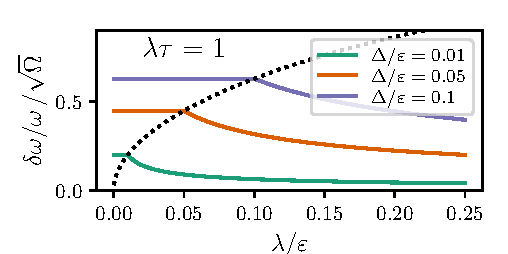
\includegraphics{gfx/Chapter04/freq_plot.pdf}
    \caption{Frequency for the optimal case $\lambda\tau=1$ for few values of $\Delta$. The black dotted curve corresponds to Eq.~(\ref{eq:freq}) for $\lambda=\Delta$}. 
    \label{fig:freqs}
\end{figure}